\documentclass[12pt, letterpaper]{article}
\usepackage[utf8]{inputenc}
\usepackage{pgfplots}

\title{Image Classification}
\author{
  Vasishta Kalinadhabhotla, Jing Yang, and Parth Mehrotra
}

\begin{document}
\maketitle
\section{Digits}
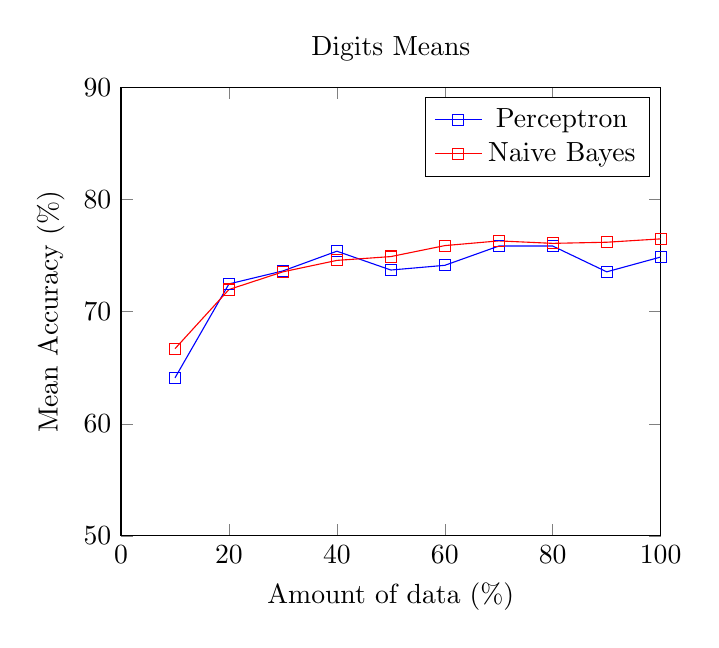
\begin{tikzpicture}
\begin{axis}[
  title={Digits Means}, 
  xlabel={Amount of data (\%)},
  ylabel={Mean Accuracy (\%)},
  xmin=0, xmax=100,
  ymin=50, ymax=90
  ]

  \addplot[
    color=blue,
    mark=square
  ]
  coordinates {
    (10, 64.1) (20, 72.47999999999999) (30, 73.64000000000001) (40, 75.39999999999999) (50, 73.72) (60, 74.14000000000001) (70, 75.86) (80, 75.86) (90, 73.55999999999999) (100, 74.88)
  };
  \addplot[
    color=red,
    mark=square
  ]
  coordinates {
    (10, 66.70000000000002) (20, 71.97999999999999) (30, 73.55999999999999) (40, 74.58) (50, 74.92) (60, 75.9) (70, 76.32000000000001) (80, 76.1) (90, 76.2) (100, 76.5)
  };
  \legend{Perceptron, Naive Bayes}

\end{axis}
\end{tikzpicture}

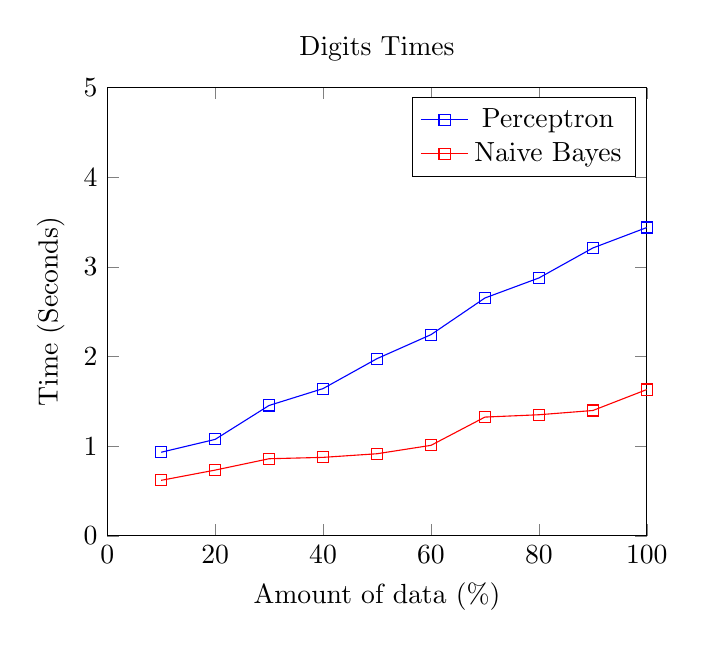
\begin{tikzpicture}
\begin{axis}[
  title={Digits Times}, 
  xlabel={Amount of data (\%)},
  ylabel={Time (Seconds)},
  xmin=0, xmax=100,
  ymin=0, ymax=5
  ]

  \addplot[
    color=blue,
    mark=square
  ]
  coordinates {
  (10,0.932571411133) (20,1.07591972351) (30,1.45445799828) (40,1.6424642086) (50,1.97654452324) (60,2.24406299591) (70,2.65311741829) (80,2.8764354229) (90,3.21098661423) (100,3.43924260139) 
  };
  \addplot[
    color=red,
    mark=square
  ]
  coordinates {
  (10,0.619478559494) (20,0.733560180664) (30,0.860241985321) (40,0.875538825989) (50,0.916040468216) (60,1.00955305099) (70,1.32490859032) (80,1.35088400841) (90,1.3982530117) (100,1.63210082054) 
  };
  \legend{Perceptron, Naive Bayes}

\end{axis}
\end{tikzpicture}

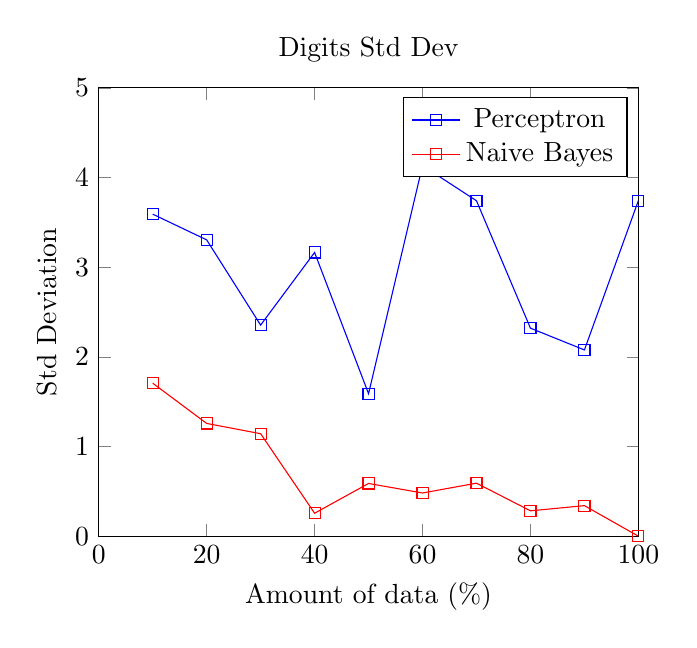
\begin{tikzpicture}
\begin{axis}[
  title={Digits Std Dev}, 
  xlabel={Amount of data (\%)},
  ylabel={Std Deviation},
  xmin=0, xmax=100,
  ymin=0, ymax=5
  ]

  \addplot[
    color=blue,
    mark=square
  ]
  coordinates {
  (10,3.59165699921) (20,3.30478441052) (30,2.35423023513) (40,3.1641744579) (50,1.58921364203) (60,4.13308601411) (70,3.74090898045) (80,2.32) (90,2.07711338159) (100,3.74240564343) 
  };
  \addplot[
    color=red,
    mark=square
  ]
  coordinates {
  (10,1.70645832062) (20,1.25761679378) (30,1.14297856498) (40,0.256124969497) (50,0.587877538268) (60,0.481663783152) (70,0.591269819964) (80,0.282842712475) (90,0.340587727319) (100,0.0) 
  };
  \legend{Perceptron, Naive Bayes}

\end{axis}
\end{tikzpicture}

\section{Faces}
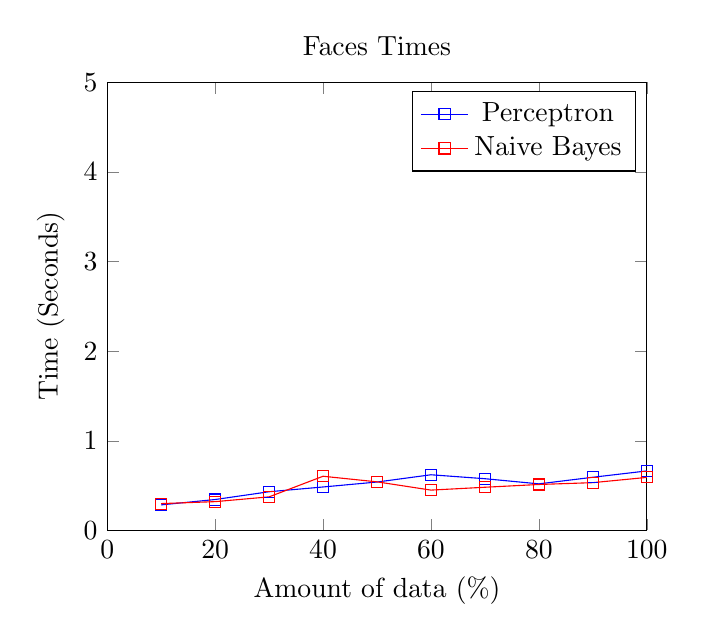
\begin{tikzpicture}
\begin{axis}[
  title={Faces Times}, 
  xlabel={Amount of data (\%)},
  ylabel={Time (Seconds)},
  xmin=0, xmax=100,
  ymin=0, ymax=5
  ]


  \addplot[
    color=blue,
    mark=square
  ]
  coordinates {
  (10,0.285628843307) (20,0.345379066467) (30,0.432191228867) (40,0.485308027267) (50,0.540548801422) (60,0.621487379074) (70,0.57750377655) (80,0.520122432709) (90,0.593709373474) (100,0.664348363876) 
  };
  \addplot[
    color=red,
    mark=square
  ]
  coordinates {
  (10,0.299941968918) (20,0.321775722504) (30,0.375074672699) (40,0.604894018173) (50,0.542614173889) (60,0.450457572937) (70,0.482290029526) (80,0.513176774979) (90,0.533605384827) (100,0.592084550858) 
  };
  \legend{Perceptron, Naive Bayes}

\end{axis}
\end{tikzpicture}

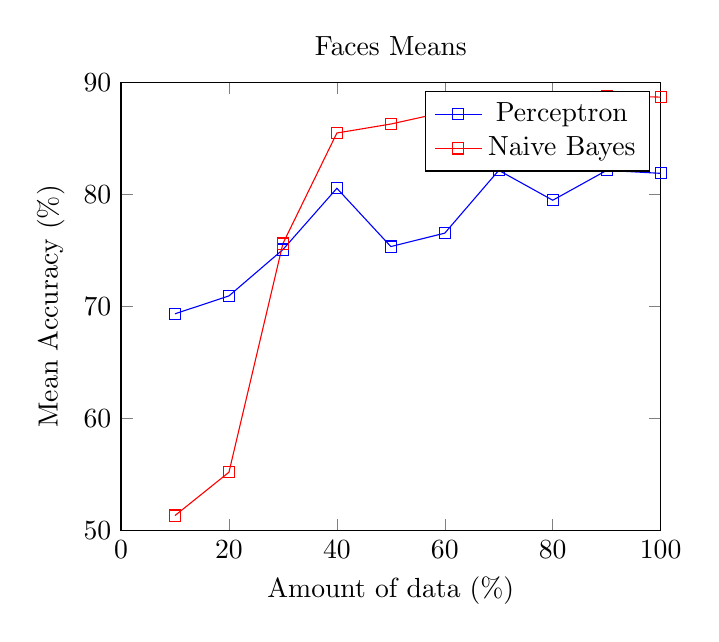
\begin{tikzpicture}
\begin{axis}[
  title={Faces Means}, 
  xlabel={Amount of data (\%)},
  ylabel={Mean Accuracy (\%)},
  xmin=0, xmax=100,
  ymin=50, ymax=90
  ]

  \addplot[
    color=blue,
    mark=square
  ]
  coordinates {
  (10,69.3333333333) (20,70.9333333333) (30,75.0666666667) (40,80.5333333333) (50,75.3333333333) (60,76.5333333333) (70,82.1333333333) (80,79.4666666667) (90,82.1333333333) (100,81.8666666667) 
  };
  \addplot[
    color=red,
    mark=square
  ]
  coordinates {
  (10,51.3333333333) (20,55.2) (30,75.6) (40,85.4666666667) (50,86.2666666667) (60,87.3333333333) (70,87.7333333333) (80,87.7333333333) (90,88.8) (100,88.6666666667) 
  };
  \legend{Perceptron, Naive Bayes}

\end{axis}
\end{tikzpicture}

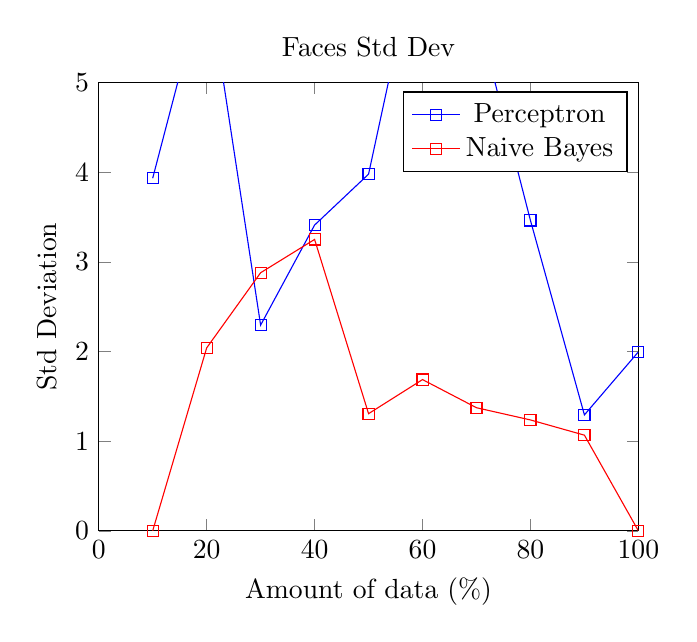
\begin{tikzpicture}
\begin{axis}[
  title={Faces Std Dev}, 
  xlabel={Amount of data (\%)},
  ylabel={Std Deviation},
  xmin=0, xmax=100,
  ymin=0, ymax=5
  ]

  \addplot[
    color=blue,
    mark=square
  ]
  coordinates {
  (10,3.932768321) (20,6.23395718803) (30,2.29395340454) (40,3.40978982735) (50,3.97771570405) (60,6.76461381012) (70,5.80268137253) (80,3.46153466287) (90,1.29271462864) (100,1.99555060628) 
  };
  \addplot[
    color=red,
    mark=square
  ]
  coordinates {
  (10,0.0) (20,2.03960780544) (30,2.87827108599) (40,3.24961536185) (50,1.30639452948) (60,1.68654808542) (70,1.37275068546) (80,1.23648246607) (90,1.06666666667) (100,0.0) 
  };
  \legend{Perceptron, Naive Bayes}

\end{axis}
\end{tikzpicture}
\section{Background}
section 1
\section{Naive Bayes Classifier}
section 1
\section{Perceptron Classifier}
section 1
\section{Discussion and Conclusions}
section 1
\end{document}
